\begin{figure}[hbp]
\centering
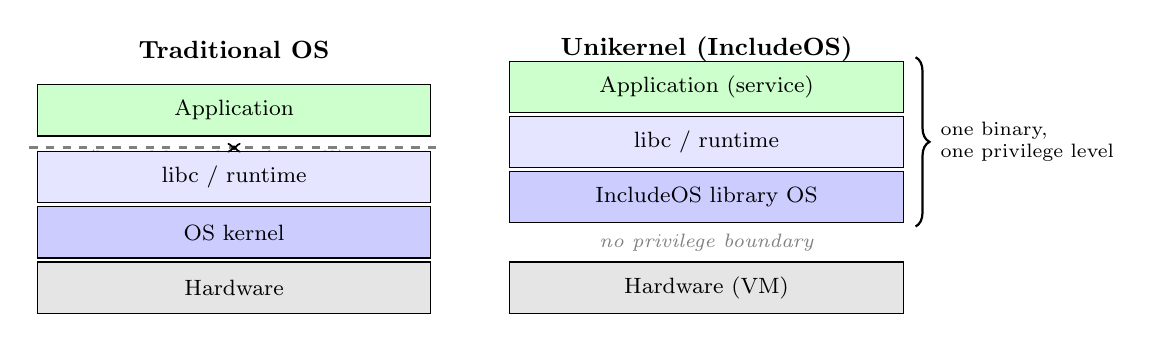
\begin{tikzpicture}[every node/.style={font=\footnotesize}]

%% ---- Left column: traditional OS ----
\node[font=\small\bfseries] at (-3.0, 5.0) {Traditional OS};

\draw[fill=green!20] (-5.5,3.9) rectangle (-0.5,4.55);
\node at (-3.0, 4.225) {Application};

%% privilege boundary
\draw[very thick, dashed, gray] (-5.6,3.75) -- (-0.4,3.75);
\node[anchor=west, font=\scriptsize\itshape, text=gray] at (-5.6,3.6)
  {user/kernel boundary (syscall)};

\draw[fill=blue!10] (-5.5,3.05) rectangle (-0.5,3.7);
\node at (-3.0, 3.375) {libc / runtime};

\draw[fill=blue!20] (-5.5,2.35) rectangle (-0.5,3.0);
\node at (-3.0, 2.675) {OS kernel};

\draw[fill=gray!20] (-5.5,1.65) rectangle (-0.5,2.3);
\node at (-3.0, 1.975) {Hardware};

%% syscall arrow
\draw[<->, thick] (-3.0,3.72) -- (-3.0,3.78);

%% ---- Right column: unikernel ----
\node[font=\small\bfseries] at (3.0, 5.0) {Unikernel (IncludeOS)};

\draw[fill=green!20]  (0.5,4.2) rectangle (5.5,4.85);
\node at (3.0, 4.525) {Application (service)};

\draw[fill=blue!10]   (0.5,3.5) rectangle (5.5,4.15);
\node at (3.0, 3.825) {libc / runtime};

\draw[fill=blue!20]   (0.5,2.8) rectangle (5.5,3.45);
\node at (3.0, 3.125) {IncludeOS library OS};

\draw[fill=gray!20]   (0.5,1.65) rectangle (5.5,2.3);
\node at (3.0, 1.975) {Hardware (VM)};

%% brace showing single binary
\draw[decorate, decoration={brace, mirror, amplitude=5pt, raise=3pt}, thick]
  (5.55, 2.75) -- (5.55, 4.90);
\node[anchor=west, align=left, font=\scriptsize] at (5.85, 3.825)
  {one binary,\\one privilege level};

%% no-boundary annotation
\node[font=\scriptsize\itshape, text=gray] at (3.0, 2.55)
  {no privilege boundary};

\end{tikzpicture}
\caption{Traditional OS vs unikernel architecture. In a conventional OS, the
  application and kernel run at different privilege levels, crossing the system
  call interface on every kernel interaction. In a unikernel, the application,
  runtime libraries, and OS library are compiled into a single binary running
  at a single privilege level. The
  dashed line is the system call boundary, which a unikernel does not have.}
\label{fig:unikernel-vs-os}
\end{figure}
